% !TeX root = ../main.tex

\section{Recursive K-Nearest Neighbors}
\subsection{Introduction}
\begin{frame}
    \frametitle{Introduction}
    \begin{columns}
        \column{0.5\textwidth}
        \begin{table}
            \centering
            \tiny
            \begin{tabular}{ |c|c|c|c|c|c|c| }
            \hline
            \diagbox{$User$}{$Item$} & \textbf{$Item_1$} & \textbf{$Item_2$} & \textbf{$Item_3$} & \textbf{$Item_4$}  & \textbf{$Item_5$} & \textbf{$Item_6$} \\
            \hline
            \textbf{$User_1$} & 5 & 2 & 3 & \textbf{?} & 1 & 5 \\
            \hline
            \textbf{$User_2$} & 1 & 2 & 4 & \textbf{?} & 2 & 2 \\
            \hline
            \textbf{$User_3$} & 4  & 3 & 5 & \textbf{?} & 4 & 3 \\
            \hline
            \textbf{$User_4$} & 5 & 2 & 3 &  \textbf{?} & \textbf{?} & \textbf{?} \\
            \hline
            \textbf{$User_5$} & \textbf{?} & \textbf{?}  & \textbf{?} & 4 & 1 & 1 \\
            \hline
            \textbf{$User_6$} & \textbf{?} & \textbf{?} & \textbf{?}  & 3 & 5 & 2 \\
            \hline
            \textbf{$User_7$} & \textbf{?} & \textbf{?} & \textbf{?}  & 5 & 1 & 2 \\
            \hline
            \textbf{$User_8$} & \textbf{?} & \textbf{?} & \textbf{?}  & 5 & 4 & 4 \\
            \hline
            \end{tabular}
            \caption{Ratings Matrix}
        \end{table}
        \column{0.5\textwidth}
        \vspace{-5mm}
        \begin{figure}
            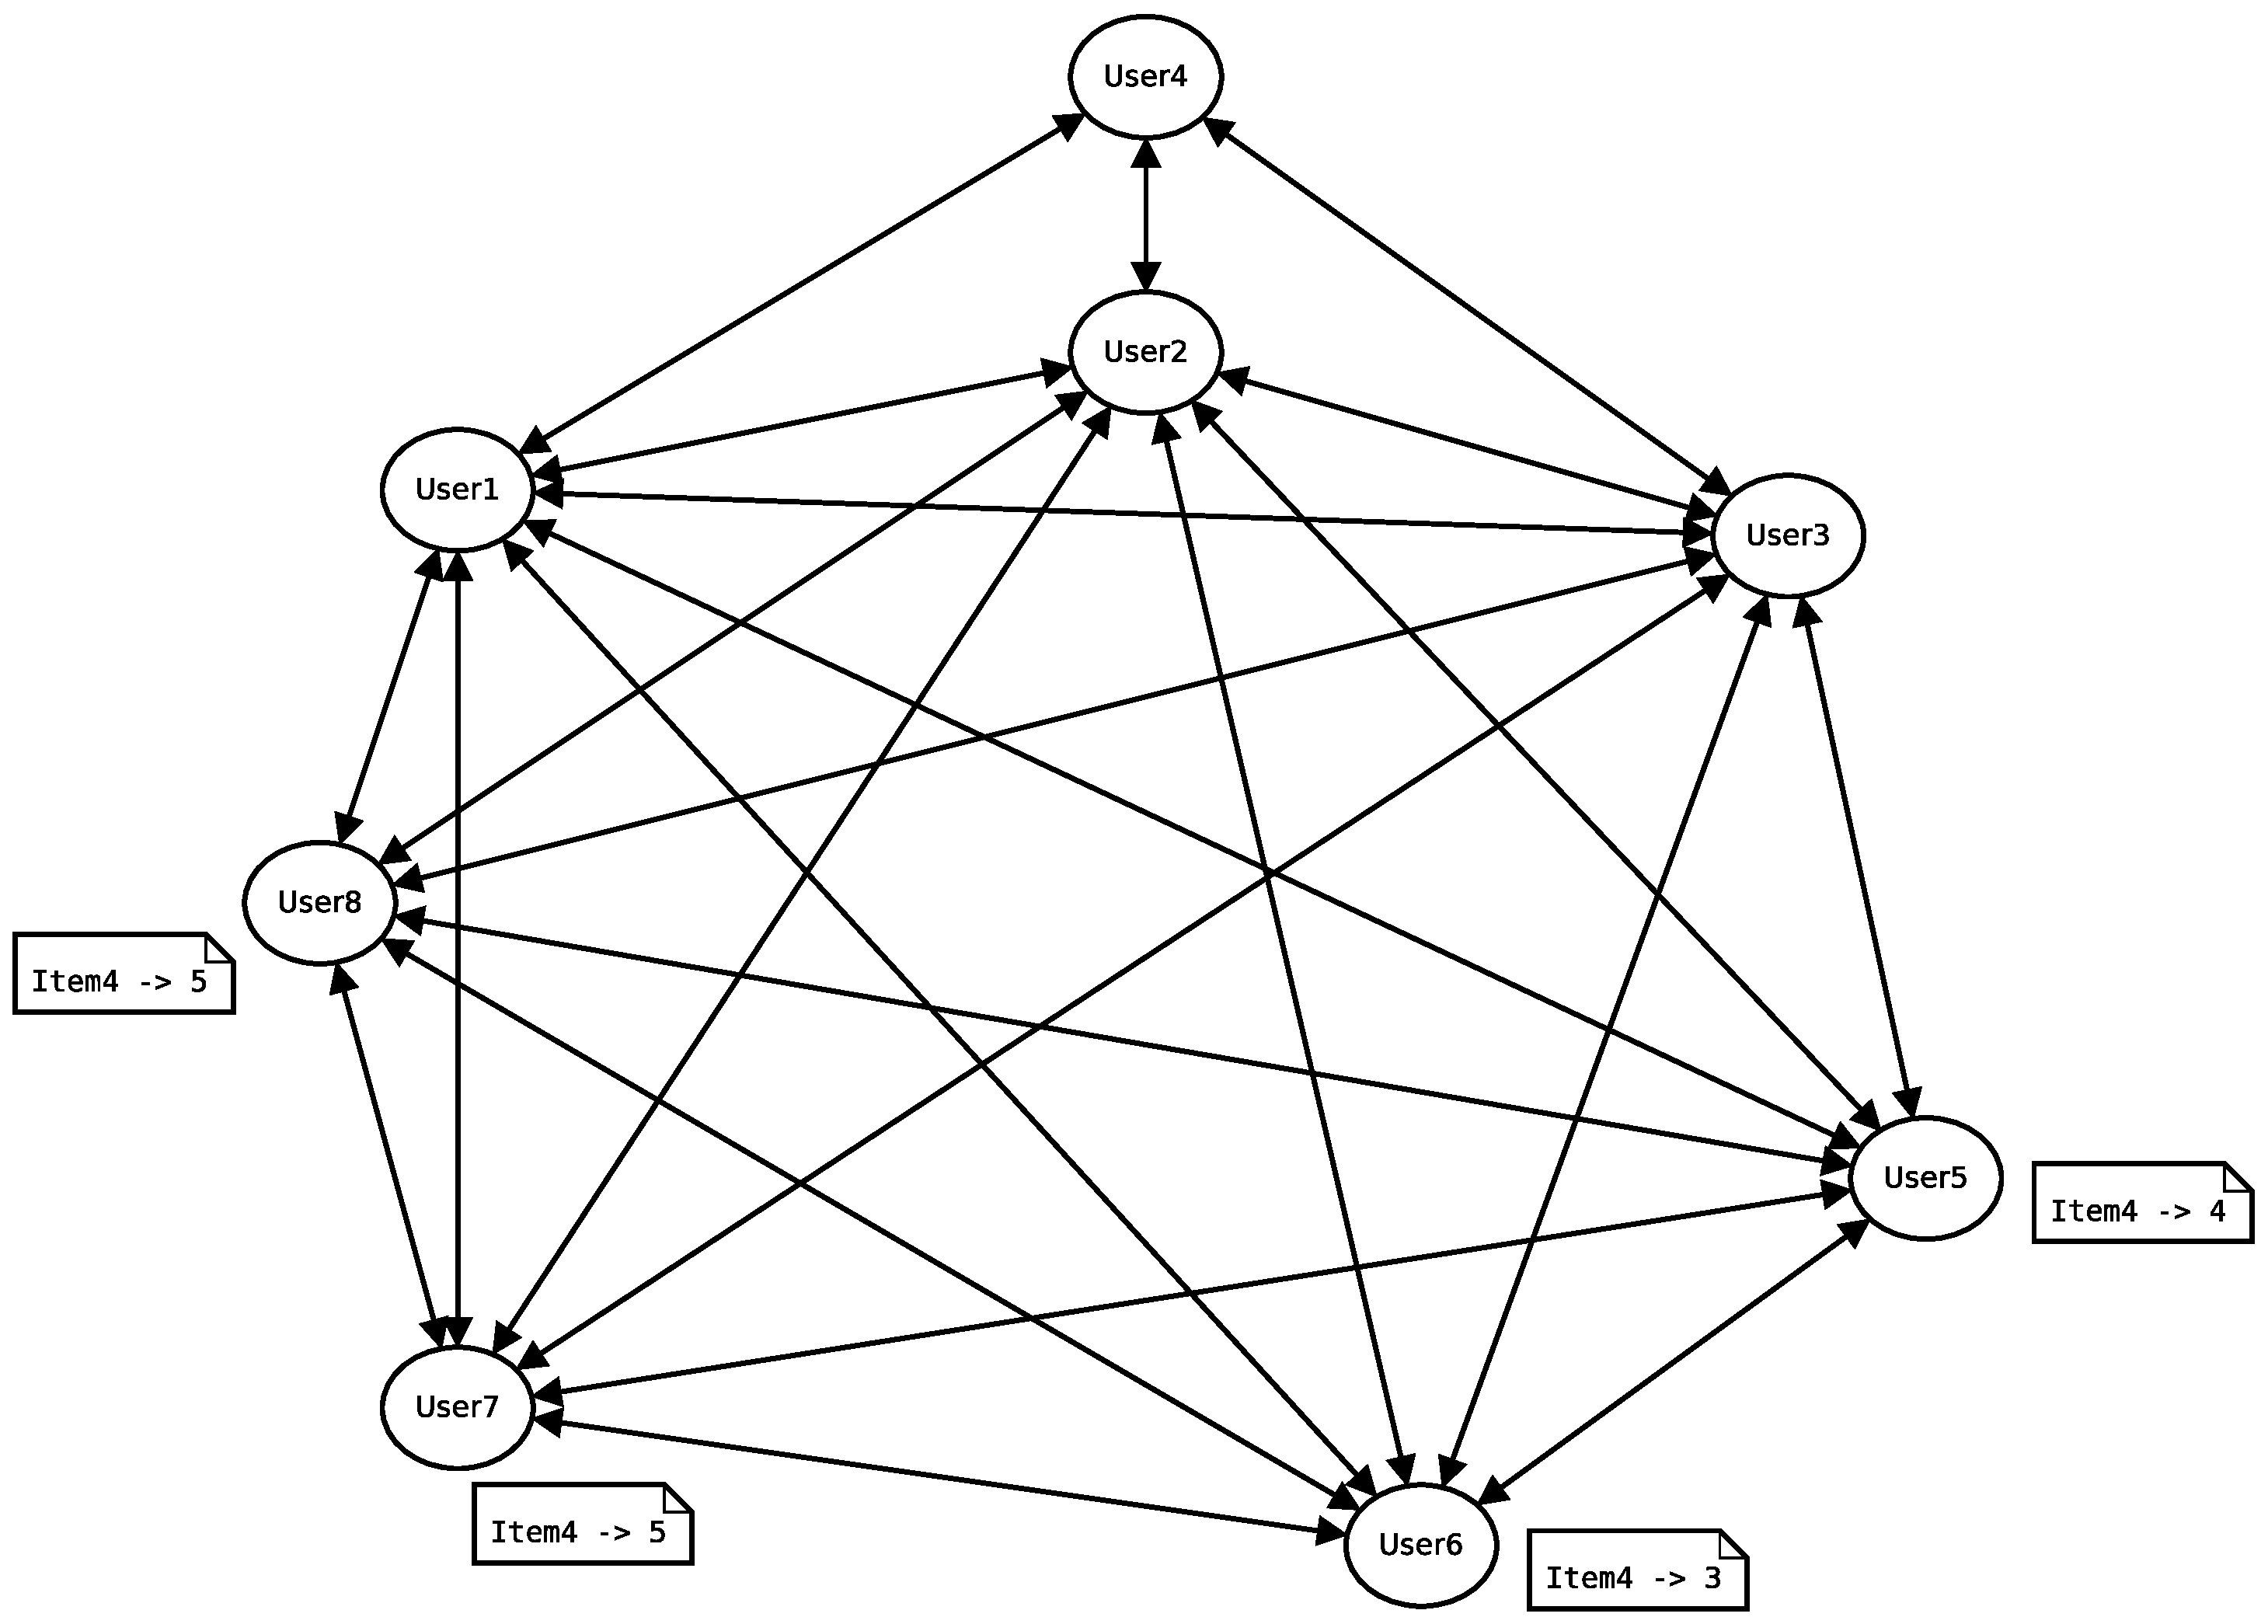
\includegraphics[width=0.95\textwidth]{user_connections.eps}
            \caption{User Connections}
        \end{figure}
    \end{columns}
\end{frame}
\begin{frame}
    \frametitle{Introduction}
    \begin{columns}
        \column{0.5\textwidth}
        \begin{table}
            \centering
            \tiny
            \begin{tabular}{ |c|c|c|c|c|c|c| }
            \hline
            \diagbox{$User$}{$Item$} & \textbf{$Item_1$} & \textbf{$Item_2$} & \textbf{$Item_3$} & \textbf{$Item_4$}  & \textbf{$Item_5$} & \textbf{$Item_6$} \\
            \hline
            \textbf{$User_1$} & 5 & 2 & 3 & {\color{red}4.3} & 1 & 5 \\
            \hline
            \textbf{$User_2$} & 1 & 2 & 4 & {\color{red}4.15} & 2 & 2 \\
            \hline
            \textbf{$User_3$} & 4  & 3 & 5 & {\color{red}4.12} & 4 & 3 \\
            \hline
            \textbf{$User_4$} & 5 & 2 & 3 &  {\color{green}\textbf{?}} & {\color{red}2.35} & {\color{red}3.42} \\
            \hline
            \textbf{$User_5$} & {\color{red}3.35} & {\color{red}2.35}  & {\color{red}4.02} & 4 & 1 & 1 \\
            \hline
            \textbf{$User_6$} & {\color{red}3.21} & {\color{red}2.4} & {\color{red}4.15}  & 3 & 5 & 2 \\
            \hline
            \textbf{$User_7$} & {\color{red}3.46} & {\color{red}2.32} & {\color{red}3.94}  & 5 & 1 & 2 \\
            \hline
            \textbf{$User_8$} & {\color{red}3.36} & {\color{red}2.35} & {\color{red}4.03}  & 5 & 4 & 4 \\
            \hline
            \end{tabular}
            \caption{Ratings Matrix After KNN}
        \end{table}
        \column{0.5\textwidth}
        \vspace{-5mm}
        \begin{figure}
            \includegraphics[width=0.95\textwidth]{user_connections_with_KNN.eps}
            \caption{User Connections}
        \end{figure}
    \end{columns}
\end{frame}
\subsection{Methodology}
\begin{frame}
    \frametitle{The Recursive K-Nearest Neighbors Algorithm}
    \only<1>{
        \vspace{2cm}
        \centering
        \textbf{The Recursive K-Nearest Neighbors algorithm}
    }
    \vspace{-1cm}
    \begin{itemize}
    \item[]<2-> \textbf{Step 1:} Select users that have similarity connections with $User_A$, name it $Group_A$.
    \item[]<3-> \textbf{Step 2:} Out of $Group_A$, select those users that have similarity connections with
	other users who have rated $Item_B$, name it $Group_B$.
    \item[]<4-> \textbf{Step 3:}  Sort $Group_B$ in descending order.
    \item[]<5-> \textbf{Step 4:}  Choose how many neighbors from $Group_B$ will contribute in the
	rating prediction by selecting the top $\mathcal{K}$ out of all the available
	neighbors in this group, name it $Group_C$.
    \item[]<6-> \textbf{Step 5:} For each neighbor in $Group_C$, predict how this neighbor would
	rate $Item_B$ using the KNN algorithm. For convenience, call the number of recursive
	neighbors each neighbor in $Group_C$ uses, $\mathcal{M}$-Nearest Neighbors.
    \item[]<7-> \textbf{Step 6:} Perform the KNN algorithm for $User_A$ to $Item_B$
    using the rating predictions applied on $Group_C$.
\end{itemize}
\end{frame}
\begin{frame}
    \frametitle{The Recursive K-Nearest Neighbors Algorithm}
    \vspace{-1cm}
    \begin{columns}
        \column{0.5\textwidth}
        \begin{figure}
        \centering
        \includegraphics[width=1\textwidth]{RKNN_prediction.eps}
        \end{figure}
        \column{0.5\textwidth}
        \begin{figure}
        \centering
        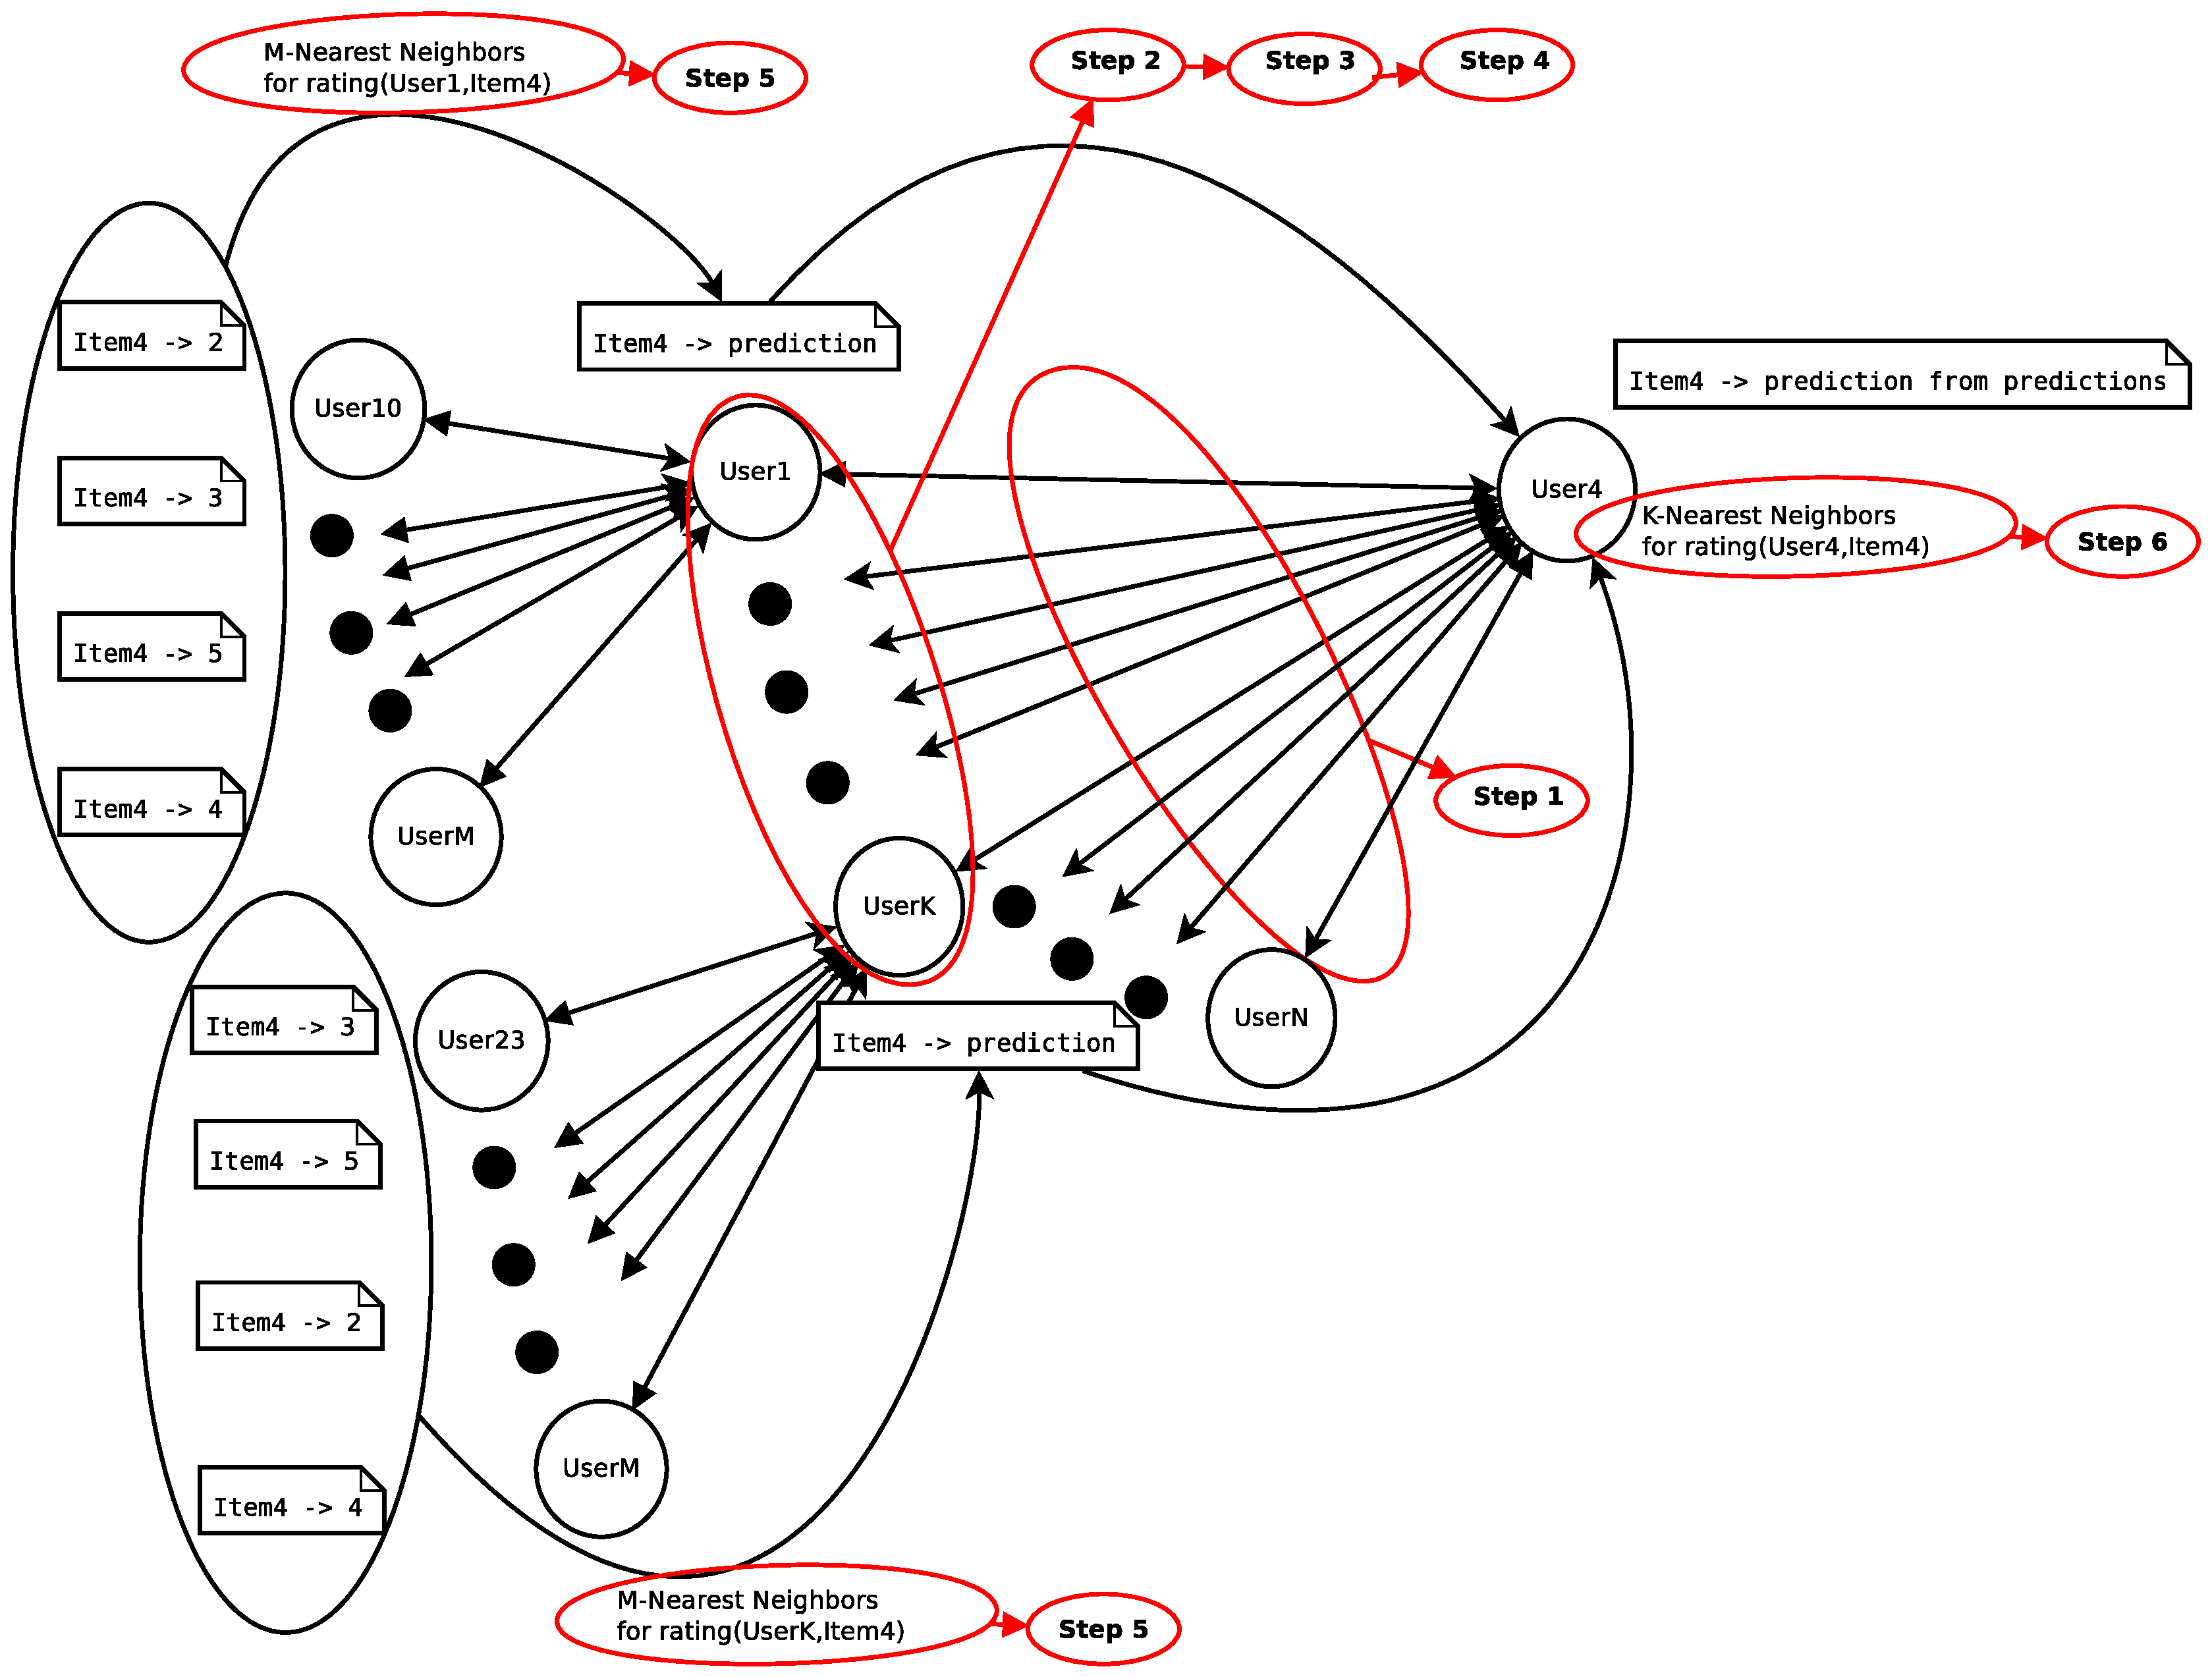
\includegraphics[width=1\textwidth]{Recursive_Nearest_Neighbors.eps}
        \end{figure}
    \end{columns}

\end{frame}
